\documentclass[a4paper]{report}

%====================== PACKAGES ======================
\usepackage[top=2cm, bottom=2cm, left=2cm, right=2cm]{geometry}
\usepackage[utf8]{inputenc}
\usepackage[T1]{fontenc}
\usepackage{amsmath,amsfonts,amssymb}

\usepackage[french]{babel}
%pour gérer les positionnement d'images
\usepackage{float}
\usepackage{array}
\usepackage{enumitem}
\usepackage{multirow}
\usepackage{mathpazo}
\usepackage{multicol}
\usepackage{nicefrac}
\usepackage{graphicx, epsfig}
\usepackage[colorinlistoftodos]{todonotes}
\usepackage{url}
%pour les informations sur un document compilé en PDF et les liens externes / internes
\usepackage{hyperref}
%pour la mise en page des tableaux
\usepackage{array}
\usepackage{tabularx}
%pour utiliser \floatbarrier
%\usepackage{placeins}
%\usepackage{floatrow}
%espacement entre les lignes
\usepackage{setspace}
%modifier la mise en page de l'abstract
\usepackage{abstract}
%police et mise en page (marges) du document
\usepackage[T1]{fontenc}
\usepackage[top=2cm, bottom=2cm, left=2cm, right=2cm]{geometry}
%Pour les galerie d'images
\usepackage{subfig}
\usepackage{placeins}

%====================== INFORMATION ET REGLES ======================

%rajouter les numérotation pour les \paragraphe et \subparagraphe
\setcounter{secnumdepth}{4}
\setcounter{tocdepth}{4}

\hypersetup{							% Information sur le document
pdfauthor = {AARAB Maryam,
			BENELKATER Mohamed,
			CORRIOU Alexandre,
    		PREVOT Alexia},			% Auteurs
pdftitle = {PROCESSUS DE DÉCISION MARKOVIEN
Un cas particulier : Homer VS Donuts},			% Titre du document
pdfsubject = {Mémoire de Projet},		% Sujet
pdfkeywords = {Tag1, Tag2, Tag3, ...},	% Mots-clefs
pdfstartview={FitH}}					% ajuste la page à la largueur de l'écran
%pdfcreator = {MikTeX},% Logiciel qui a crée le document
%pdfproducer = {}} % Société avec produit le logiciel

%======================== DEBUT DU DOCUMENT ========================

\begin{document}

%régler l'espacement entre les lignes
\newcommand{\HRule}{\rule{\linewidth}{0.5mm}}

%page de garde
\begin{titlepage}
\begin{center}

% Upper part of the page. The '~' is needed because only works if a paragraph has started.

\includegraphics[width=0.35\textwidth]{./Logo_Polytech_Sorbonne}~\\[1cm]
\includegraphics[width=0.35\textwidth]{./Logo_Sorbonne_Université}~\\[1cm]

\textsc{\Large }\\[0.5cm]

% Title
\HRule \\[0.4cm]

{\huge \bfseries Projet\\
PROCESSUS DE DÉCISION MARKOVIEN\\
Un cas particulier : Homer VS Donuts \\[0.4cm] }

\HRule \\[1.5cm]


\includegraphics[width=0.35\textwidth]{./donut}~\\[1cm]

% Author and supervisor
\begin{minipage}{0.4\textwidth}
\begin{flushleft} \large
AARAB \textsc{Maryam}\\
BENELKATER \textsc{Mohamed}\\
CORRIOU \textsc{Alexandre}\\
PREVOT \textsc{Alexia}
\end{flushleft}
\end{minipage}
\begin{minipage}{0.4\textwidth}
\begin{flushright} \large
\emph{Encadrant:} \\
Jeanne \textsc{Barthélemy}\\
\emph{MAIN3} \\
2020/2021
\end{flushright}
\end{minipage}

\vfill

% Bottom of the page
{\large \today}

\end{center}
\end{titlepage}

%page blanche
\newpage
~
%ne pas numéroter cette page
\thispagestyle{empty}

\Large
\tableofcontents
%\thispagestyle{empty}
%\setcounter{page}{0}
%ne pas numéroter le sommaire

%\newpage

%espacement entre les lignes d'un tableau
\renewcommand{\arraystretch}{1.5}

%====================== INCLUSION DES PARTIES ======================

~
\thispagestyle{empty}
%recommencer la numérotation des pages à "1"
\setcounter{page}{0}
\newpage
\makeatletter\@addtoreset{section}{part}\makeatother
\renewcommand{\thesection}{\arabic{section}}
\normalsize
\section{Pésentation}
\vspace{0.6cm}

\subsection{Le sujet}
Dans ce projet nous devrons réaliser un code visant à aider Homer à trouver le chemin le plus court vers les donuts en
évitant les ennemis. C'est-à-dire nous devrons créer un environnement, des actions et des récompenses en fonction de la position dans l'environnement. Pour cela, nous devrons utiliser le processus de décision markovien et ainsi prendre en compte une part d'aléatoire dans les décisions de l'agent.
\vspace{0.6cm}

\FloatBarrier %bloque l'image dans le texte
\begin{figure}[!h]
\centering
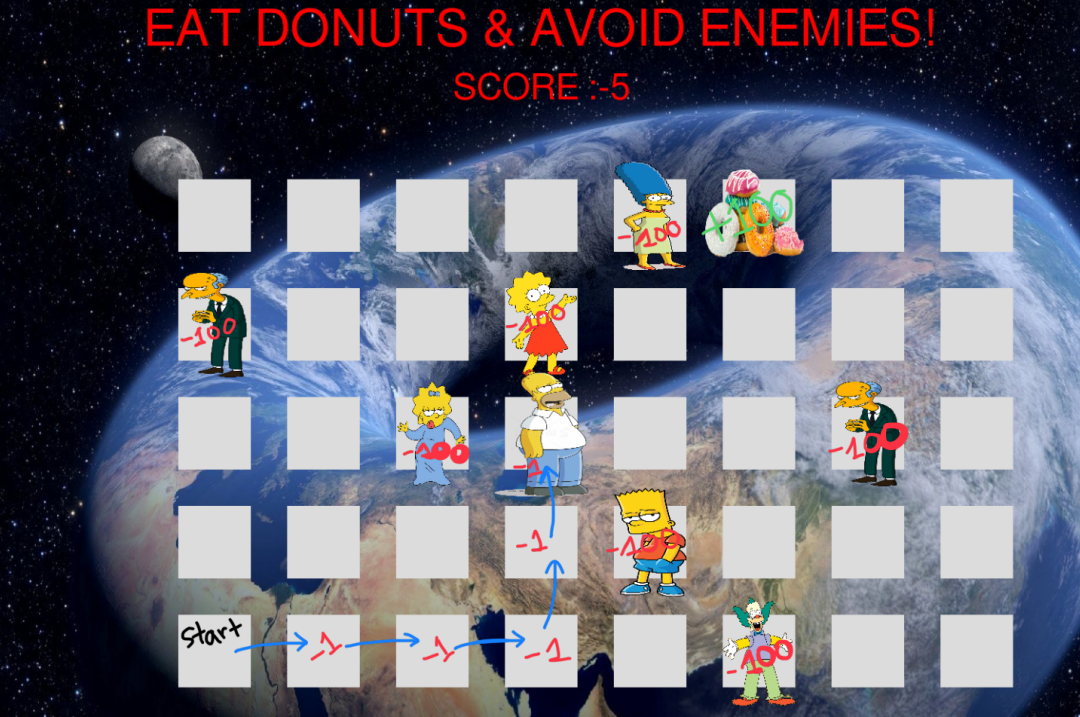
\includegraphics[width=14cm,scale=1]{Capture2.PNG}
\caption{Exemple de l'interface à obtenir}
\end{figure}
\FloatBarrier


\subsection{Problème soulevé}

D'abord, ce sujet nous laisse relativement libre et afin de commencer au mieux, notre encadrante nous a proposé des mots clés pour savoir dans quelle direction partir : 
\begin{itemize}
  \item[$\bullet$] programmation dynamique (itération de politique, itération de valeur) ;
  \item[$\bullet$] apprentissage par renforcement ; 
  \item[$\bullet$] environnement stochastique ;
  \item[$\bullet$] model based / model free ; 
  \item[$\bullet$] processus décisionnel Markovien.
\end{itemize}


Cela permet de mieux comprendre le sujet et nous guider vers ce que nous devons faire dans la suite.


\subsubsection{Programmation dynamique}
 La programmation dynamique consiste à résoudre un problème en le décomposant en sous-problèmes, puis à résoudre les sous-problèmes, des plus petits aux plus grands en stockant les résultats intermédiaires.
 
\subsubsection{Apprentissage par renforcement}

L'apprentissage par renforcement est une méthode utilisée pour créer des intelligences artificielles. On appelle \textbf{agent autonome} la machine (robot ou autre) à qui on fait subir cet apprentissage. Grâce à des expériences répétées un grand nombre de fois, l'agent cherche à maximiser la récompense qui lui est attribuée quand il réussit la tâche que l'on veut qu'il effectue.

\subsubsection{Environnement stochastique}
Un environnement stochastique est un environnement dont les paramètres évoluent de manière aléatoire. Cela s’oppose aux environnements dits déterministes. Les organismes vivant dans ces habitats variables et imprévisibles doivent donc s’adapter rapidement afin d’y survivre et de pouvoir s’y reproduire. (\href{https://fr.wikiversity.org/wiki/Adaptations_aux_environnements_stochastiques#:~:text=Un\%20environnement\%20stochastique\%20est\%20un,de\%20pouvoir\%20s'y\%20reproduire.}{Wikipédia})

\subsubsection{Modèle}
Un modèle est un environnement dans lequel un agent évolue. On sépare habituellement deux manières d'effectuer un apprentissage, désignés par les termes anglais : model based et model free.
\begin{enumerate}
\item{\underline{Model based}}\\
Dans une simulation dite "model based", l'agent peut "demander" à l'environnement quelles récompenses il obtiendra si il fait telle ou telle action, lui permettant de prédire son futur score. Pour trouver le chemin optimal, il peut donc tenter d'améliorer le plus possible son chemin pendant l'éxécution du programme.
\item{\underline{Model free}}\\
Dans une simulation dite "model free", l'agent évolue à l'aveugle et ne connait la récompense d'une action que quand il l'effectue. Pour trouver le chemin optimal, il doit donc effectuer un grand nombre de répétitions de l'expérience avant d'avoir des données suffisantes pour pouvoir savoir où aller. Ce genre de modèles n'est régi que par l'aléatoire, contrairement au précédent.
\end{enumerate}

\subsubsection{Processus décisionnel Markovien}

Dans notre projet, l'objectif sera d'entraîner un modèle afin qu'à l'issue de l'entraînement, Homer trouve le plus court chemin jusqu'aux donuts et ainsi que le problème soit résolu.

Il existe différents types d'apprentissage afin d'entraîner notre modèle. \\
Mais tout d'abord il faut modéliser le problème et pour cela nous allons utiliser un processus décisionnel markovien (MDP). Un MDP est un quadruplet \{ S , A , T , R \} qui définit : 
\begin{itemize}
  \item[$\bullet$] \textbf{S} : qui représente l'ensemble les états d'un environnement ;
  \item[$\bullet$] \textbf{A} : l'ensemble des actions applicable dans notre environnement à savoir les déplacements de Homer d'une case à l'autre (haut, bas, droite, gauche) ; 
  \item[$\bullet$] \textbf{T} : la fonction probabilité de transition qui définis la probabilité que Homer passe d'un état à un autre en fonction de l'action appliqué ;
  \item[$\bullet$] \textbf{R} : la fonction qui associe chaque état de l'environnement à une récompense (case vide : SCORE - 1, case avec ennemi :  SCORE - 100, case avec donuts  : SCORE + 100).
\end{itemize}


\newpage
\section{Mode de travail}

\vspace{0.6cm}

\subsection{Espace de travail}
Nous avons très rapidement mis en place un espace de travail pour être au plus efficace :

\begin{itemize}
  \item[$\bullet$]création d'un drive commun pour se partager des documents. Nous avons déjà un document qui nous servira à noter à chaque séance nos avancées et ainsi cela permet d'une part de se rendre compte de où nous en sommes et d'une autre part nous permettra vers la fin du projet de garder les dates et l'ordre de nos avancées ;
  \item[$\bullet$] création d'un serveur discord afin de faciliter la discussion et le partage d'information rapidement comme des liens de sites internet ou autres. De plus, si besoin nous pourrons alors faire des réunions à distance et parler dans des salons vocaux facilement ; 
  \item[$\bullet$] création d'un espace git afin de partager nos codes. 
  (\href{https://github.com/viitality/Homer-vs-Donuts}{Lien Github})
  
\end{itemize}

\vspace{0.6cm}

\subsection{Organisation du travail}

Nous sommes mis d'accord avec le groupe pour se retrouver chaque mercredi après-midi en présentiel afin d'avancer sur le projet et éventuellement discuter de nos avancées personnelles concernant le travail. Néanmoins, en cas de d'indisponibilité, nous organiserons des réunions Zoom en distanciel.
\\

Pour la mise en place d'un bon environnement de travail, nous suivons les valeurs suivantes afin de mener à bien les objectifs et d'avoir une bonne entente de groupe :
\begin{itemize}
\item[$\bullet$] motivation, c'est un sujet qui nous intéresse et on doit se donner à fond pour le mener à bien ;
\item[$\bullet$] esprit d’équipe, c'est un travail de groupe avant tout comme on pourrait avoir plus tard dans la vie professionnelle alors savoir travailler en équipe sera inévitable ;
\item[$\bullet$] communication, nécessaire pour se comprendre et partager les informations ;
\item[$\bullet$] efficacité, comme avait dit Bill Gates : "Je choisis une personne paresseuse pour un travail difficile, car une personne paresseuse va trouver un moyen facile de le faire", c'est-à-dire que notre travail doit être clair et efficace (passer des heures sur un problème ne signifie pas qu'il sera bien résolu) ;
\item[$\bullet$] confiance, puisque l'on va se répartir des tâches, il faut apprendre à faire confiance à ses camarades pour travailler efficacement en équipe ;
\item[$\bullet$] respect, cela paraît évidant mais on doit respecter notre encadrante mais aussi chaque personne du projet ;
\item[$\bullet$] etc.
\end{itemize}

\part{Début du travail, d'un point de vue théorique et/ou numérique}


\newpage
\section{Conclusion}

\vspace{1 cm}

Ainsi, ce projet fait intervenir de nombreuses notions de mathématiques, de machine learning, d'inforamtique et autres. Notre objectif principale pour le moment sera de chercher un moyen d'apprentissage pour résoudre notre problème et trouver le chemin le plus optimisé afin maximiser le score. Par la suite nous pourrons améliorer les interfaces graphiques pour afficher le score par exemple et enfin en fonction de notre avancement, nous pourrons réfléchir à un modèle plus complexe de ce jeu comme par exemple le positionement aléatoire des agents au début de partie.


%récupérer les citation avec "/footnotemark"
\nocite{*}

%choix du style de la biblio
\bibliographystyle{plain}
%inclusion de la biblio
\bibliography{Bibliographie.bib}
%voir wiki pour plus d'information sur la syntaxe des entrées d'une bibliographie


\end{document}